\chapter{CVN}
\label{chap:cvn}

Here are some funky floats using ``continued captions'', i.e. for a semantically
collected group of float contents which are too numerous to fit into a single
float, such as the pretty circles in the following figure

\section{Convolutional Neural Networks}
\label{sec:cnn}

\section{CHIPS Events}
\label{sec:events}

\begin{comment}
    TODO: test todo
\end{comment}

\begin{figure}
    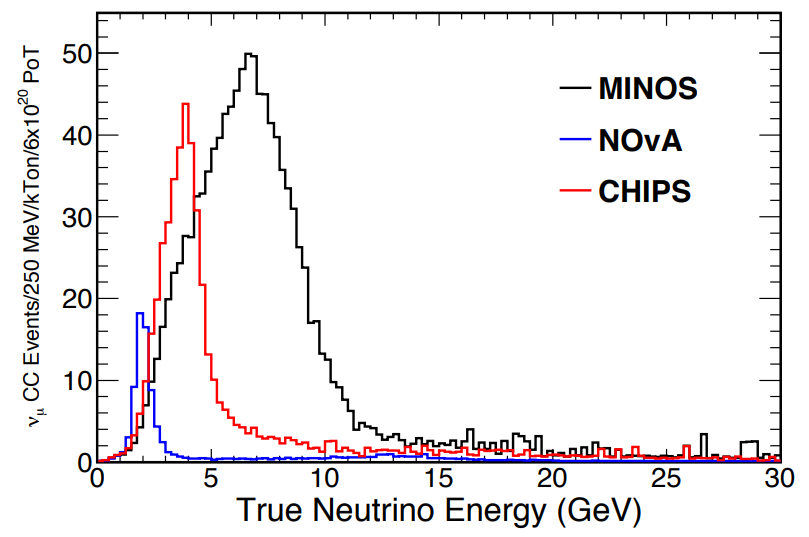
\includegraphics[width=\largefigwidth]{diagrams/cvn/numi_axis}
    \caption[numi_axis]%
    {blah blah blah chips chips chips lots or very exciting caption content.}
    \label{fig:numi_axis}
\end{figure}

\begin{figure}
    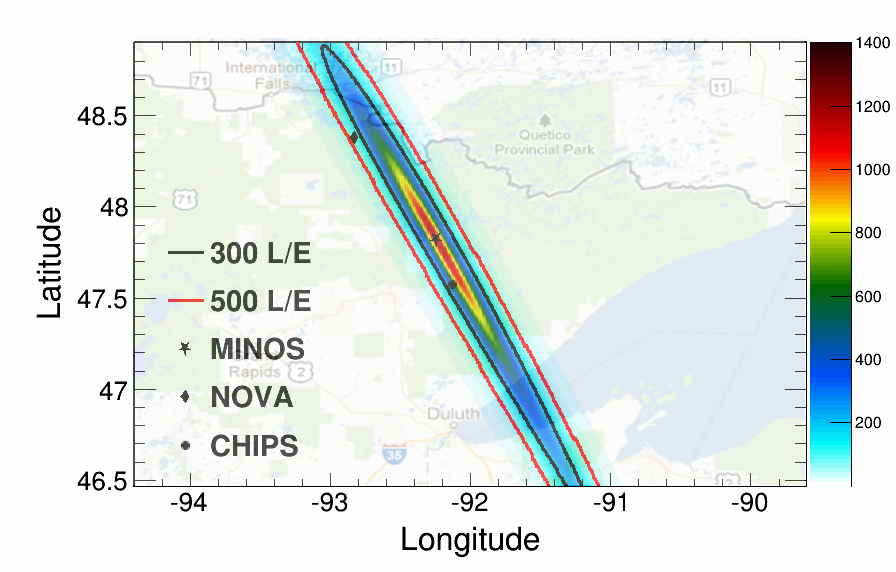
\includegraphics[width=\largefigwidth]{diagrams/cvn/numi_map}
    \caption[numi_map]%
    {blah blah blah chips chips chips lots or very exciting caption content.}
    \label{fig:numi_map}
\end{figure}

\begin{figure}
    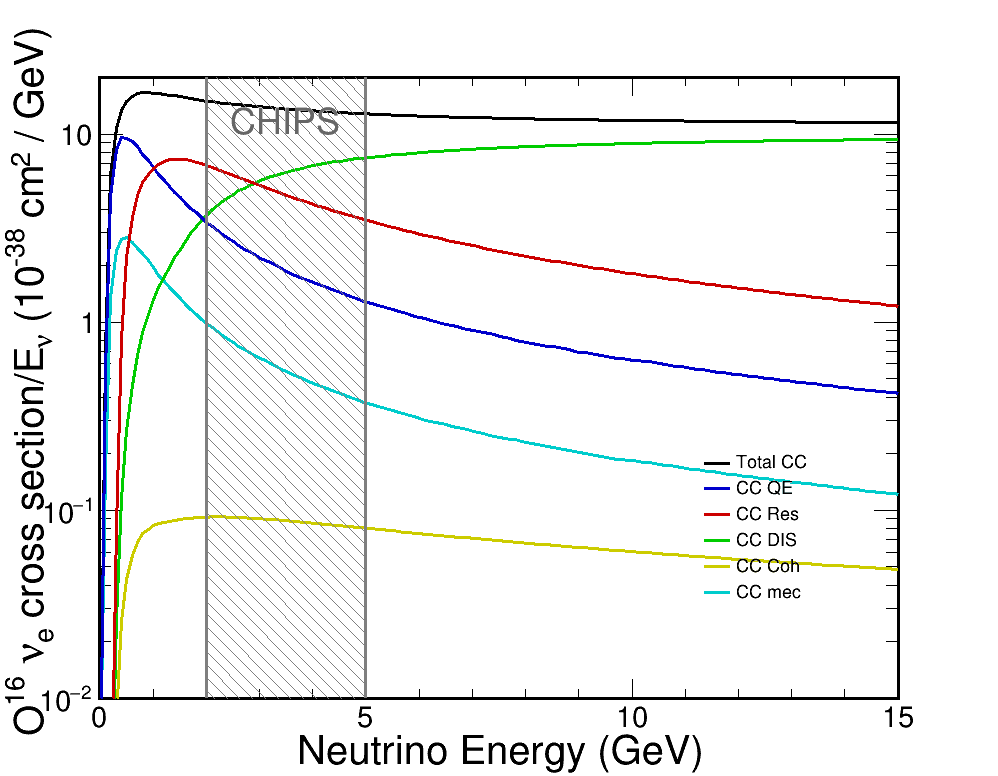
\includegraphics[width=\largefigwidth]{diagrams/cvn/xsec_cc_nu_e_O16}
    \caption[xsec_cc_nu_e_O16]%
    {blah blah blah chips chips chips lots or very exciting caption content.}
    \label{fig:xsec_cc_nu_e_O16}
\end{figure}

\begin{figure}
    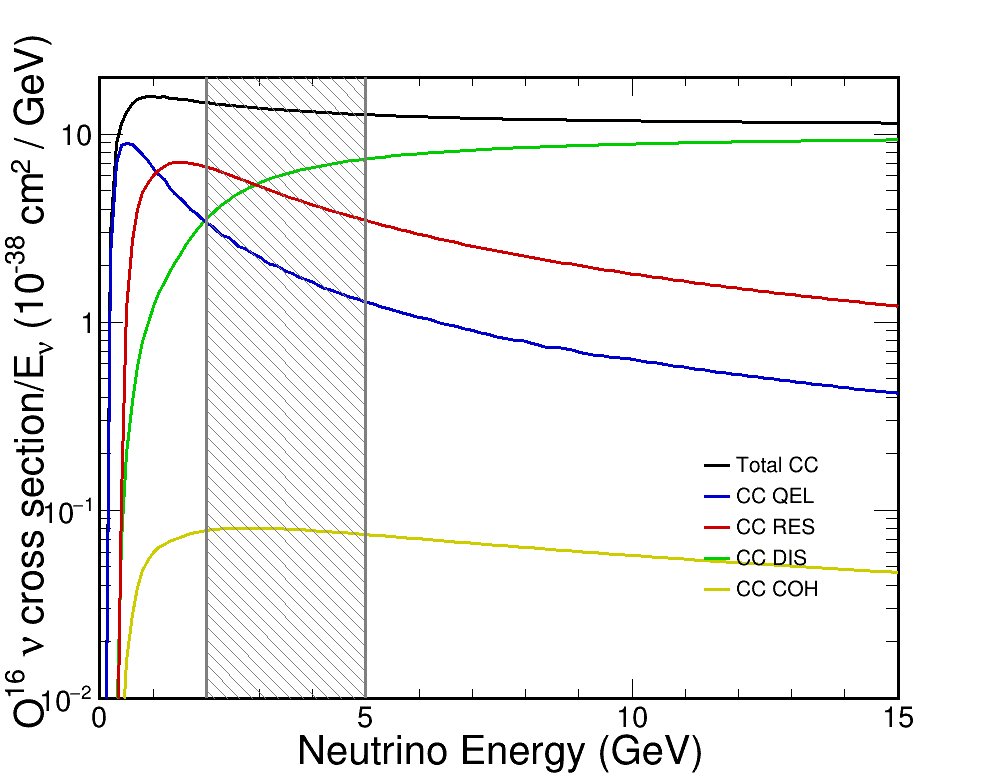
\includegraphics[width=\largefigwidth]{diagrams/cvn/xsec_cc_nu_mu_O16}
    \caption[xsec_cc_nu_mu_O16]%
    {blah blah blah chips chips chips lots or very exciting caption content.}
    \label{fig:xsec_cc_nu_mu_O16}
\end{figure}

\begin{figure}
    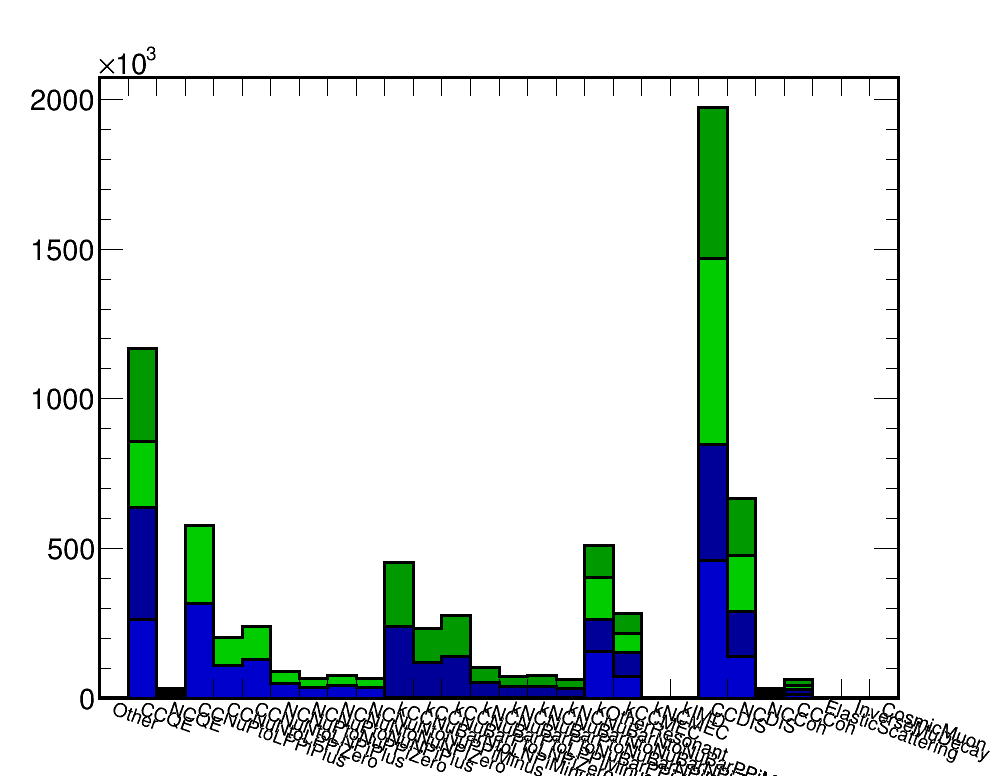
\includegraphics[width=\largefigwidth]{diagrams/cvn/events}
    \caption[events]%
    {blah blah blah chips chips chips lots or very exciting caption content.}
    \label{fig:events}
\end{figure}

\begin{figure}
    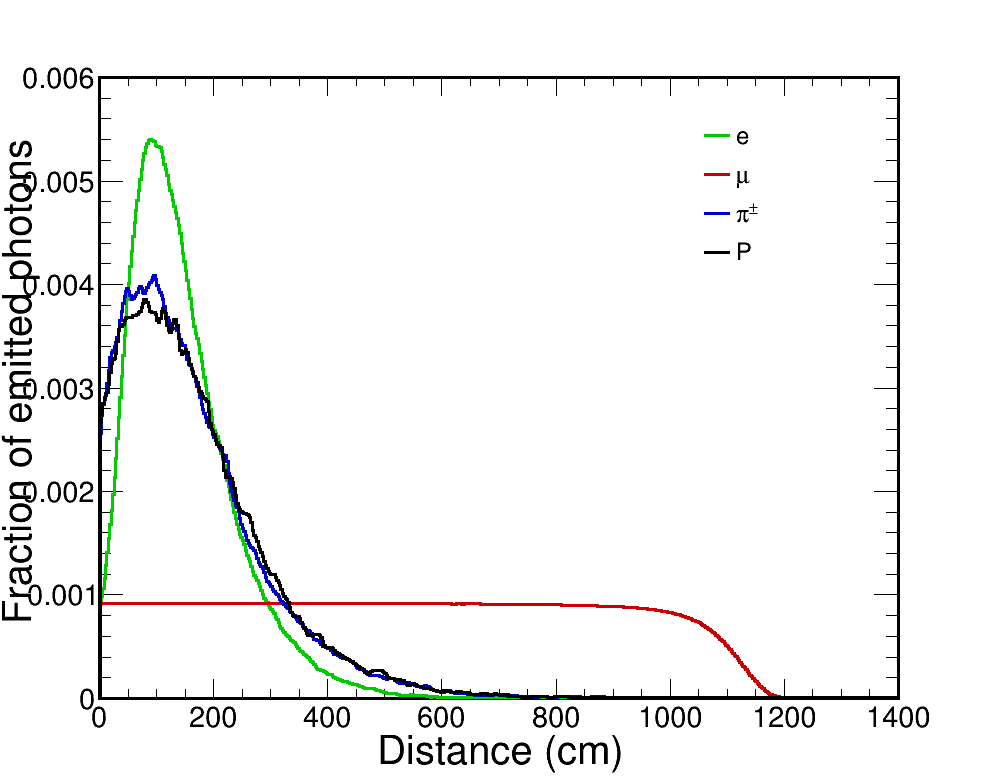
\includegraphics[width=\largefigwidth]{diagrams/cvn/emission_distance}
    \caption[emisson_distance]%
    {blah blah blah chips chips chips lots or very exciting caption content.}
    \label{fig:emisson_distance}
\end{figure}

\begin{figure}
    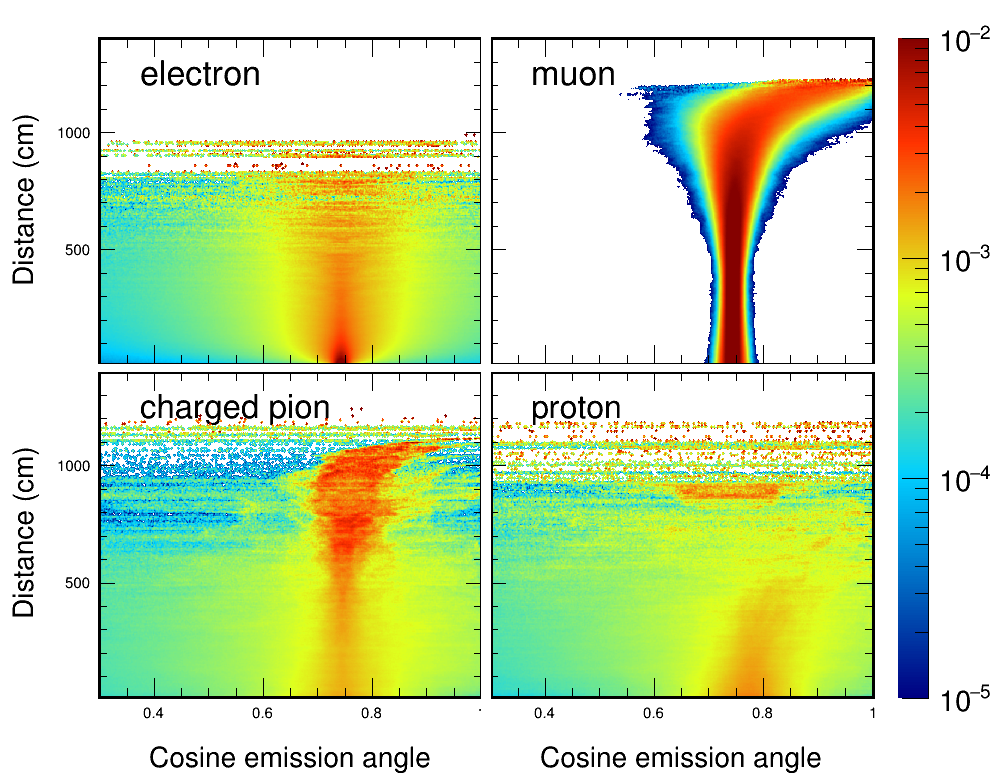
\includegraphics[width=\largefigwidth]{diagrams/cvn/emission_profile}
    \caption[emisson_profile]%
    {blah blah blah chips chips chips lots or very exciting caption content.}
    \label{fig:emisson_profile}
\end{figure}

\begin{figure}
    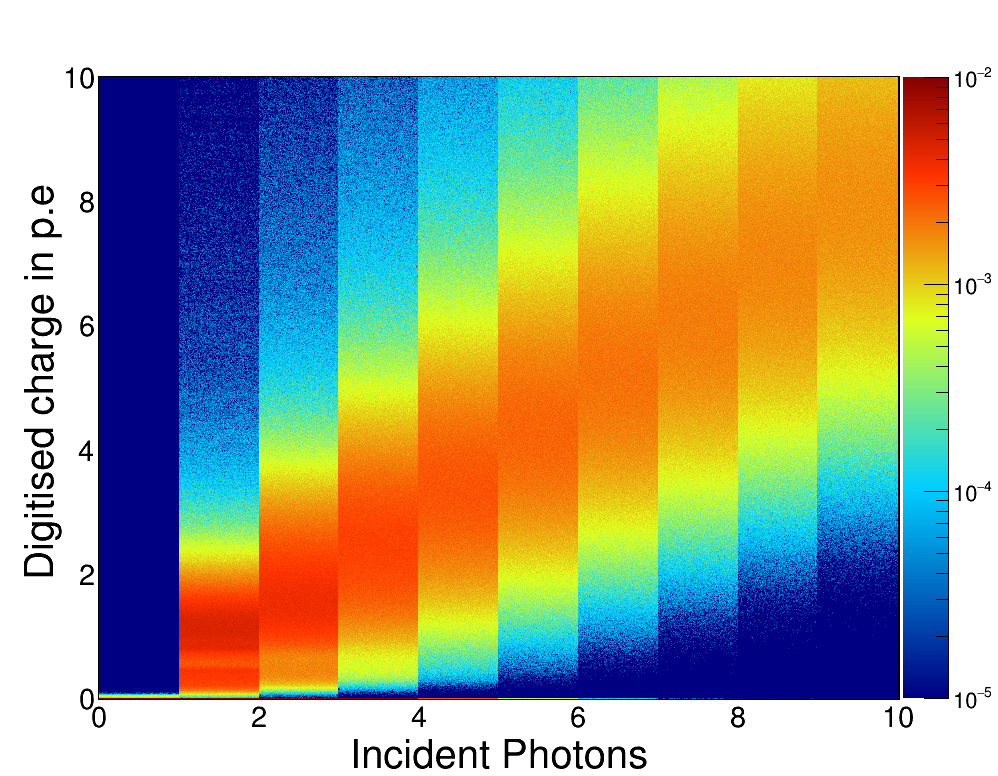
\includegraphics[width=\largefigwidth]{diagrams/cvn/digi_method}
    \caption[digi_method]%
    {blah blah blah chips chips chips lots or very exciting caption content.}
    \label{fig:digi_method}
\end{figure}

\begin{figure}
    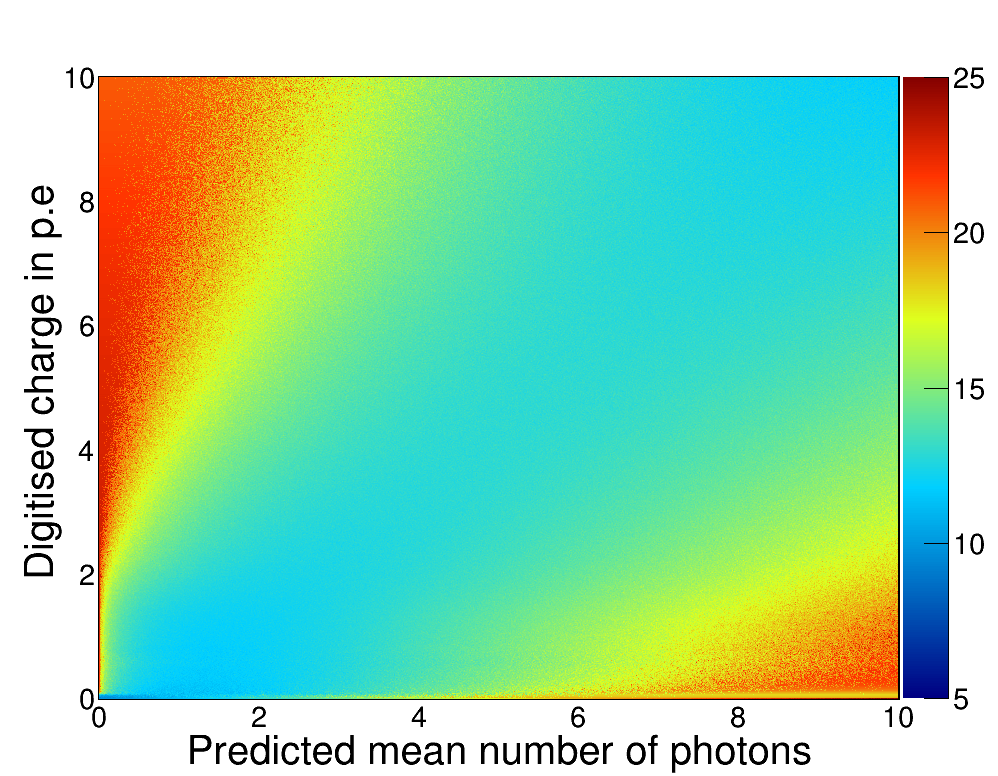
\includegraphics[width=\largefigwidth]{diagrams/cvn/digi_likelihood}
    \caption[digi_likelihood]%
    {blah blah blah chips chips chips lots or very exciting caption content.}
    \label{fig:digi_likelihood}
\end{figure}

The expected beam flux at the CHIPS detector location is found from reweighting current

We can use current NuMI beam simulations

Current NuMI beam experiments

